\documentclass[tikz,border=6pt]{standalone}
\usepackage[T1]{fontenc}
\usepackage[utf8]{inputenc}
\usepackage{pgfplots}
\usepgfplotslibrary{groupplots}
\usetikzlibrary{calc}
\pgfplotsset{compat=1.18}
\begin{document}
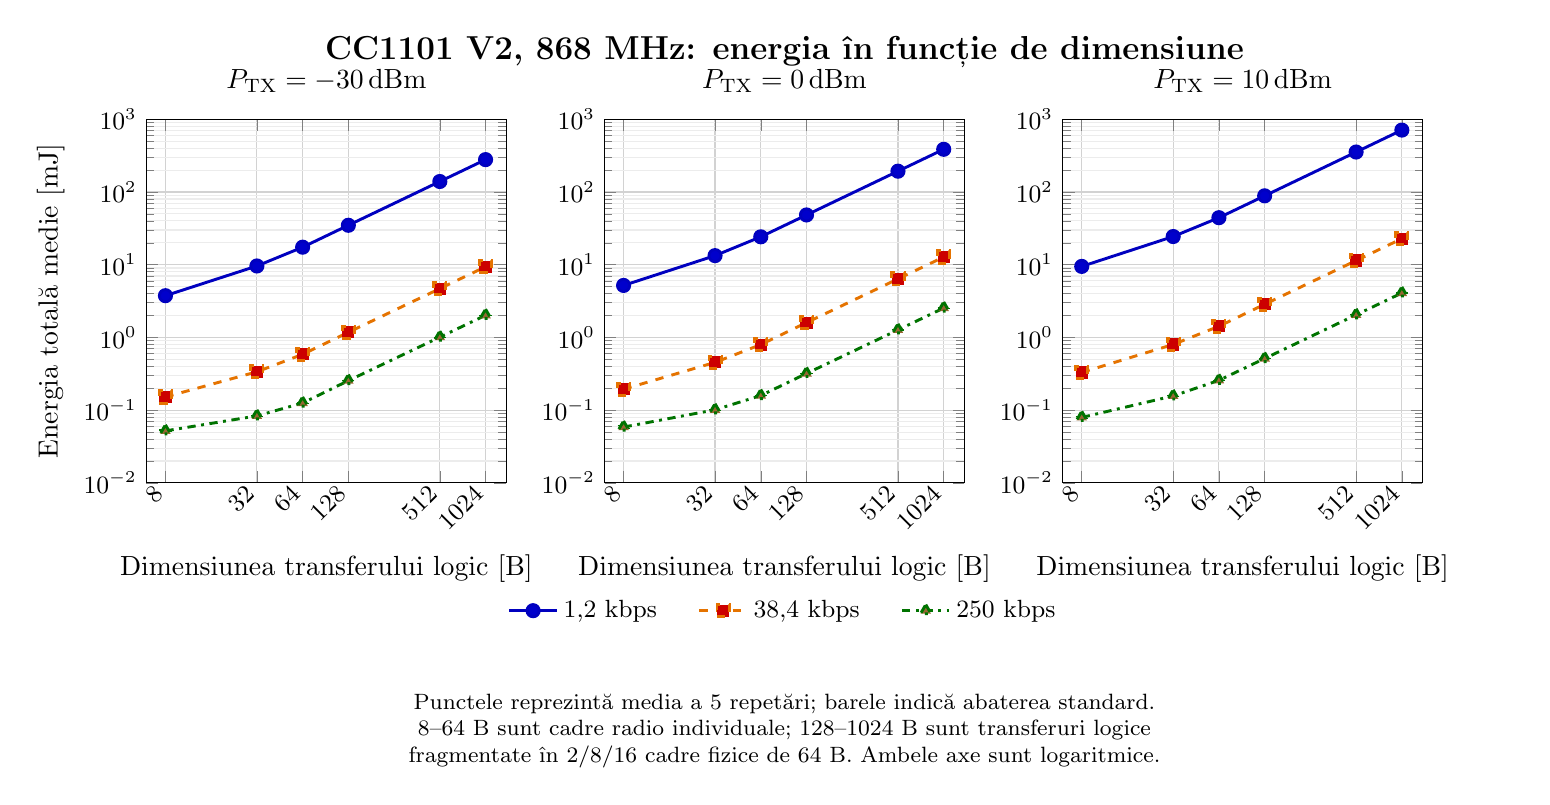
\begin{tikzpicture}
\begin{groupplot}[/pgf/number format/use comma,
  group style={group size=3 by 1, horizontal sep=1.25cm},
  width=6.15cm, height=6.2cm,
  xmode=log, log basis x={2},
  ymode=log, log basis y={10},
  ymin=0.01, ymax=1000,
  xmin=6, xmax=1400,
  xtick={8,32,64,128,512,1024},
  xticklabels={8,32,64,128,512,1024},
  x tick label style={rotate=45, anchor=east, font=\small},
  y tick label style={font=\small},
  grid=both, minor grid style={gray!15}, major grid style={gray!35},
  xlabel={Dimensiunea transferului logic [B]},
  every axis plot/.append style={line width=1.05pt},
  error bars/error bar style={line width=0.35pt},
  legend style={font=\small, draw=none, fill=none,
    at={(0.5,-0.29)}, anchor=north, legend columns=3,
    /tikz/every even column/.append style={column sep=0.45cm}},
]
\nextgroupplot[title={\(P_{\mathrm{TX}}=-30\,\mathrm{dBm}\)}, ylabel={Energia totală medie [mJ]}]
\addplot+[
  color=blue!75!black, solid, mark=*, mark size=2.2pt,
  error bars/.cd, y dir=both, y explicit,
] coordinates {
  (8,3.75169734) +- (0,0.0105523914)
  (32,9.6071812) +- (0,0.0082319855)
  (64,17.4174964) +- (0,0.00761950385)
  (128,34.8636326) +- (0,0.0845158583)
  (512,139.326726) +- (0,0.0489718422)
  (1024,278.607541) +- (0,0.210416727)
};
\addplot+[
  color=orange!90!black, dashed, mark=square*, mark size=2.2pt,
  error bars/.cd, y dir=both, y explicit,
] coordinates {
  (8,0.151898944) +- (0,0.00292564525)
  (32,0.336972764) +- (0,0.00263934137)
  (64,0.586002919) +- (0,0.00200912946)
  (128,1.17695854) +- (0,0.00357225596)
  (512,4.69226609) +- (0,0.00547469442)
  (1024,9.3727813) +- (0,0.0111009607)
};
\addplot+[
  color=green!45!black, dashdotted, mark=triangle*, mark size=2.2pt,
  error bars/.cd, y dir=both, y explicit,
] coordinates {
  (8,0.0518650955) +- (0,0.00151411779)
  (32,0.0834199408) +- (0,0.000671538028)
  (64,0.125401165) +- (0,0.00112843786)
  (128,0.254588065) +- (0,0.0015555999)
  (512,1.00874107) +- (0,0.00333609695)
  (1024,2.01835148) +- (0,0.00306536421)
};
\nextgroupplot[title={\(P_{\mathrm{TX}}=0\,\mathrm{dBm}\)}]
\addplot+[
  color=blue!75!black, solid, mark=*, mark size=2.2pt,
  error bars/.cd, y dir=both, y explicit,
] coordinates {
  (8,5.1898792) +- (0,0.00424823393)
  (32,13.3297135) +- (0,0.00581883681)
  (64,24.1857319) +- (0,0.0206466505)
  (128,48.3203487) +- (0,0.0232918365)
  (512,193.164012) +- (0,0.137246834)
  (1024,386.204039) +- (0,0.21713439)
};
\addlegendentry{1{,}2 kbps}
\addplot+[
  color=orange!90!black, dashed, mark=square*, mark size=2.2pt,
  error bars/.cd, y dir=both, y explicit,
] coordinates {
  (8,0.194268502) +- (0,0.00163718159)
  (32,0.453971757) +- (0,0.00311615687)
  (64,0.797366624) +- (0,0.00195998541)
  (128,1.59869141) +- (0,0.00254868648)
  (512,6.37953024) +- (0,0.00470134992)
  (1024,12.7537163) +- (0,0.00973005525)
};
\addlegendentry{38{,}4 kbps}
\addplot+[
  color=green!45!black, dashdotted, mark=triangle*, mark size=2.2pt,
  error bars/.cd, y dir=both, y explicit,
] coordinates {
  (8,0.0585171821) +- (0,0.00261674068)
  (32,0.101172518) +- (0,0.00153989999)
  (64,0.158668327) +- (0,0.00159931184)
  (128,0.319471125) +- (0,0.00264254082)
  (512,1.26942614) +- (0,0.00210688769)
  (1024,2.53587639) +- (0,0.00417769445)
};
\addlegendentry{250 kbps}
\nextgroupplot[title={\(P_{\mathrm{TX}}=10\,\mathrm{dBm}\)}]
\addplot+[
  color=blue!75!black, solid, mark=*, mark size=2.2pt,
  error bars/.cd, y dir=both, y explicit,
] coordinates {
  (8,9.4775302) +- (0,0.00515582437)
  (32,24.4041946) +- (0,0.00948351986)
  (64,44.3061416) +- (0,0.0123686459)
  (128,88.5760176) +- (0,0.0348137768)
  (512,354.365512) +- (0,0.200330587)
  (1024,709.569705) +- (0,0.470200464)
};
\addplot+[
  color=orange!90!black, dashed, mark=square*, mark size=2.2pt,
  error bars/.cd, y dir=both, y explicit,
] coordinates {
  (8,0.330203149) +- (0,0.00232009835)
  (32,0.80035129) +- (0,0.00166063854)
  (64,1.42389739) +- (0,0.00178019767)
  (128,2.85597755) +- (0,0.00399775026)
  (512,11.4040865) +- (0,0.00308792769)
  (1024,22.8118886) +- (0,0.00747804466)
};
\addplot+[
  color=green!45!black, dashdotted, mark=triangle*, mark size=2.2pt,
  error bars/.cd, y dir=both, y explicit,
] coordinates {
  (8,0.0795413873) +- (0,0.00205677522)
  (32,0.156821947) +- (0,0.00230282557)
  (64,0.257031598) +- (0,0.00235228998)
  (128,0.513097673) +- (0,0.00198568945)
  (512,2.04490721) +- (0,0.00259166338)
  (1024,4.08408997) +- (0,0.00197511679)
};
\end{groupplot}
\node[font=\bfseries\large] at ($(group c2r1.north)+(0,0.85cm)$)
  {CC1101 V2, 868 MHz: energia în funcție de dimensiune};
\node[font=\footnotesize, align=center, text width=18.5cm]
  at ($(group c2r1.south)+(0,-3.15cm)$)
  {Punctele reprezintă media a 5 repetări; barele indică abaterea standard.\\
   8--64 B sunt cadre radio individuale; 128--1024 B sunt transferuri logice\\
   fragmentate în 2/8/16 cadre fizice de 64 B. Ambele axe sunt logaritmice.};
\end{tikzpicture}
\end{document}
